\let\negmedspace\undefined
\let\negthickspace\undefined
\documentclass[journal]{IEEEtran}
\usepackage[a5paper, margin=10mm, onecolumn]{geometry}
\usepackage{lmodern} % Ensure lmodern is loaded for pdflatex
\usepackage{tfrupee} % Include tfrupee package

\setlength{\headheight}{1cm} % Set the height of the header box
\setlength{\headsep}{0mm}     % Set the distance between the header box and the top of the text

\usepackage{gvv-book}
\usepackage{gvv}
\usepackage{cite}
\usepackage{amsmath,amssymb,amsfonts,amsthm}
\usepackage{algorithmic}
\usepackage{graphicx}
\usepackage{textcomp}
\usepackage{xcolor}
\usepackage{txfonts}
\usepackage{listings}
\usepackage{enumitem}
\usepackage{mathtools}
\usepackage{gensymb}
\usepackage{comment}
\usepackage[breaklinks=true]{hyperref}
\usepackage{tkz-euclide} 
\usepackage{listings}
 \usepackage{gvv}                                        
\def\inputGnumericTable{}                                 
\usepackage[latin1]{inputenc}                                
\usepackage{color}                                            
\usepackage{array}                                            
\usepackage{longtable}                                       
\usepackage{calc}                                             
\usepackage{multirow}                                         
\usepackage{hhline}                                           
\usepackage{ifthen}                                           
\usepackage{lscape}
\begin{document}

\bibliographystyle{IEEEtran}


\title{4.10.23}
\author{EE25BTECH11021 - Dhanush Sagar}

{\let\newpage\relax\maketitle}

\renewcommand{\thefigure}{\theenumi}
\renewcommand{\thetable}{\theenumi}
\setlength{\intextsep}{10pt} % Space between text and floats
\numberwithin{equation}{enumi}
\numberwithin{figure}{enumi}
\renewcommand{\thetable}{\theenumi}
\textbf{Question} \\
Find the equation of the line passing through the point of intersection of 2x + y = 5
and x + 3y + 8 = 0 and parallel to the line 3x + 4y = 7.



\bigskip
\noindent \textbf{Solution:}
The two given lines are written in matrix form as
\begin{align}
l_1 = \myvec{2 \\ 1}\vec{x} &= 5, \\
l_2 = \myvec{1 \\ 3}\vec{x} &= -8.\\
l_3 = \myvec{3 \\ 4}\vec{x} &= 7. \\
\end{align}
\noindent{\small Normals and constants for the given lines $l_1$ and $l_2$.}
\begin{align}
\vec{n}_1 &= \myvec{2\\1}, \quad c_1=5 \\
\vec{n}_2 &= \myvec{1\\3}, \quad c_2=-8
\end{align}
\noindent{\small General family of lines through the intersection, written as $l_1+\lambda l_2$.}

\begin{align}
(\vec{n}_1^T\vec{x}-c_1) + \lambda(\vec{n}_2^T\vec{x}-c_2) &= 0
\end{align}

\noindent{\small Explicit expanded form of the family of lines.}
\begin{align}
\myvec{2 & 1}\vec{x}-5 + \lambda\big(\myvec{1 & 3}\vec{x}+8\big) &= 0 \\
\implies \myvec{2+\lambda & 1+3\lambda}\vec{x} &= 5 - 8\lambda.  
\end{align}



Normal of the line $l_3$, to which our required line must be parallel.


\begin{align}
\vec{m} &= \myvec{3\\4}
\end{align}

\noindent{\small Normal vector of the family of lines.}

\begin{align}
\vec{N}(\lambda) &= \vec{n}_1 + \lambda\vec{n}_2 = \myvec{2+\lambda\\1+3\lambda}
\end{align}
\noindent{\small Condition for parallelism with $\vec{m}$.}
\begin{align}
\vec{N}(\lambda) &= \alpha\vec{m}
\implies \myvec{2+\lambda\\1+3\lambda} = \alpha\myvec{3\\4}
\end{align}

\noindent{\small Solve these equations to determine $\lambda$.}

\begin{align}
3\alpha - \lambda &= 2 \\
4\alpha - 3\lambda &= 1
\end{align}

\begin{align}
\myvec{3 & -1 & \vline & 2 \\ 4 & -3 & \vline & 1}
\end{align}

\begin{align}
R_1 &\to \tfrac{1}{3}R_1 \\
\myvec{3 & -1 & \vline & 2 \\ 4 & -3 & \vline & 1} 
&\;\Rightarrow\;
\myvec{1 & -\tfrac{1}{3} & \vline & \tfrac{2}{3} \\ 4 & -3 & \vline & 1}
\end{align}

\begin{align}
R_2 &\to R_2 - 4R_1 \\
\myvec{1 & -\tfrac{1}{3} & \vline & \tfrac{2}{3} \\ 4 & -3 & \vline & 1}
&\;\Rightarrow\;
\myvec{1 & -\tfrac{1}{3} & \vline & \tfrac{2}{3} \\ 0 & -\tfrac{5}{3} & \vline & -\tfrac{5}{3}}
\end{align}

\begin{align}
R_2 &\to \left(-\tfrac{3}{5}\right)R_2 \\
\myvec{1 & -\tfrac{1}{3} & \vline & \tfrac{2}{3} \\ 0 & -\tfrac{5}{3} & \vline & -\tfrac{5}{3}}
&\;\Rightarrow\;
\myvec{1 & -\tfrac{1}{3} & \vline & \tfrac{2}{3} \\ 0 & 1 & \vline & 1}
\end{align}

\begin{align}
R_1 &\to R_1 + \tfrac{1}{3}R_2 \\
\myvec{1 & -\tfrac{1}{3} & \vline & \tfrac{2}{3} \\ 0 & 1 & \vline & 1}
&\;\Rightarrow\;
\myvec{1 & 0 & \vline & 1 \\ 0 & 1 & \vline & 1}
\end{align}

\begin{align}
\lambda &= 1
\end{align}

substituting value of $\lambda$ in eq(0.9) .Final equation of the required line in matrix form.
\begin{align}
\myvec{3 & 4}\vec{x} + 3 &= 0
\end{align}

\begin{figure}[H]
    \centering
    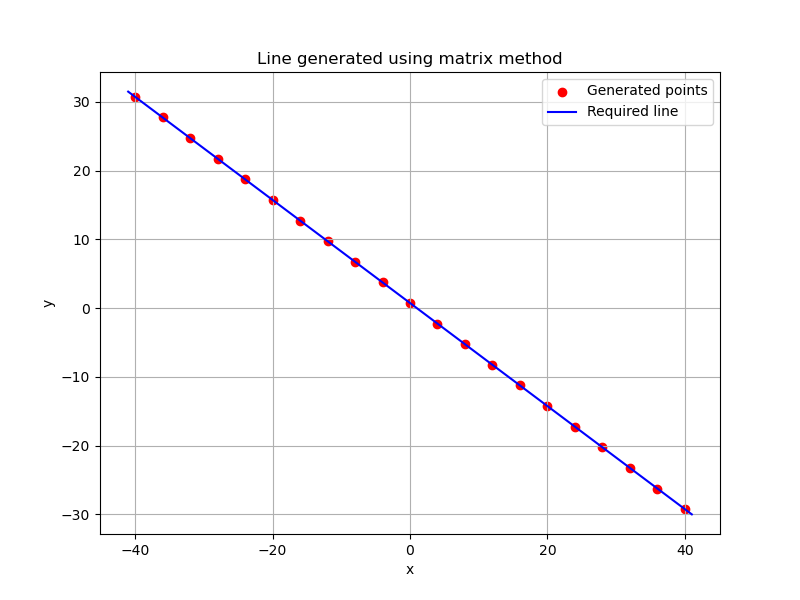
\includegraphics[width=0.5\columnwidth]{figs/fig1.png}
    \caption{}
    \label{fig:placeholder}
\end{figure}
\end{document}

